\section{Results}
\label{sec:results}
\subsection{Confirmatory tests}
The confirmation run comprises \sNrowsConf{} filter runs on \sNconf{} trajectories. Table~\ref{tab:s3tests} gives the prespecified tests and Table~\ref{tab:s3main} the trajectory level medians by level; Fig.~\ref{fig:s3res} plots the main systems.

\textbf{H1 is supported.} With dust coupled to the image visibility, bias and an untuned noise model, the DoP weighted compass B3 lowers the heading RMSE from \sHoneB{} to \sHoneA{} degrees (median over trajectories of the mean over D0, D2 and D4; paired difference \sHonediff{} degrees, cluster bootstrap interval [\sHonelo{}, \sHonehi{}]). The gain grows with the degradation: at D4 the heading RMSE falls from \scBzeroDfourhd{} to \scBthreeDfourhd{} degrees and the drift from \scBzeroDfourdr{} to \scBthreeDfourdr{} percent of path length.

\textbf{H2 is supported.} The confirmation poses are level, so H2 was tested with a heading bias and no tilt: an ungated fixed weight compass is worse than none even with clear images, with a heading RMSE at D0 of \sHtwoA{} degrees against \sHtwoB{} for B0 (in the tilt sensitivity run, \stBoneDzerohd{} against \stBzeroDzerohd{}). In the 21 June 11:45 and 12:30 scenarios, pooled over levels, its run level mean heading RMSE is \snoonBonePooled{} degrees (\snoonBoneDzero{} at D0).

\textbf{H3 (equivalently H3b, since S = B4) is supported.} The selected scheme S (B4, the DoP floored covariance matching that was exploratory in Study~2) is not worse than covariance matching B2 (difference \sHthreediff{} degrees, interval [\sHthreelo{}, \sHthreehi{}], margin 0.5). The new robust, two mode, bias state and learned schemes (B5 to B8) lie within about 0.2 degrees of B3 and B4 when the three levels are pooled (Table~\ref{tab:s3main}); the bias state B7 is the best compass scheme at D0 (\scBsevenDzerohd{} against \scBthreeDzerohd{} degrees), where the bias dominates, and the worst of them at D4.

\textbf{H4 is supported.} Adding the ring of off zenith points (B4R) lowers the heading RMSE from \sHfourB{} to \sHfourA{} degrees (difference \sHfourdiff{}, interval [\sHfourlo{}, \sHfourhi{}]). The confirmation poses carry no tilt, however; on the development split, with an assumed 2 degree tilt, the ring did not help (B4R tied B4 and B3R was worse than B3, because the sharper ring noise estimate made the gate reject tilted samples; Section~\ref{sec:tilt}).

\textbf{H5 is supported.} Without any camera, SIMULATED wheel odometry with the zenith compass (W3) drifts \sHfiveA{} percent at D4 against \sHfiveB{} percent for stereo VO without a compass (difference \sHfivediff{}, interval [\sHfivelo{}, \sHfivehi{}]); with the ring compass (W4R) the drift is lower still. The ant's combination of a stride integrator and a sky compass outperforms severely degraded vision in this setting; it depends on the assumed wheel slip model, and with clear images on the development split vision was better (B0 \sdevBzeroDzerodr{} against W3 \sdevWthreeDzerodr{} percent at D0).

\textbf{H6 and H7 are not met.} The calibrated noise model B3C does not repair consistency: its median position NEES is \sHsixNees{} (B3: \sHsixNeesBthree{}) and its mean 95 percent coverage \sHsixCov{} (B3: \sHsixCovBthree{}), far from the band [1, 4] and [0.8, 0.99]; it also raised the drift at D0 from \scBthreeDzerodr{} to \scBthreeCDzerodr{} percent. The ranking of the VO systems on the development split does not transfer (Kendall $\tau$ = \sHseventau{}): the weighted schemes lie within a few tenths of a degree of each other, so their order is not stable, while the gross order (ring and weighted schemes, then the gated fixed weight, then no compass, then the ungated fixed weight) is.

\begin{table*}[t]
\caption{Study 3 confirmatory tests (confirmation split, \sNconf{} trajectories, coupled dust sky). $A$ and $B$: medians over trajectories; Diff: median paired difference $A-B$ with a two stage cluster bootstrap 95 percent interval; $p$: one sided Wilcoxon, Holm over H1, H2, H4 and H5; H3 and H3b are non inferiority tests with a margin of 0.5 degrees on the upper bound.}
\label{tab:s3tests}
\centering\footnotesize
\begin{tabular}{llrrrrl}
\toprule
H & Pair & $A$ & $B$ & Diff [95\% CI] & $p_{\mathrm{Holm}}$ & Result \\
\midrule
H1 & B3$-$B0 (D0,D2,D4) & 1.98 & 5.10 & -3.15$^\circ$ [-5.27, -1.10] & $<$0.001 & yes \\
H2 & B1$-$B0 (D0) & 7.66 & 1.72 & 5.73$^\circ$ [0.01, 7.43] & $<$0.001 & yes \\
H3, H3b & B4$-$B2 (D0,D2,D4) & 2.11 & 2.04 & 0.01$^\circ$ [-0.02, 0.11] & -- & yes \\
H4 & B4R$-$B4 (D0,D2,D4) & 1.40 & 2.11 & -0.71$^\circ$ [-1.01, -0.42] & $<$0.001 & yes \\
H5 & W3$-$B0 (D4) & 1.22 & 3.46 & -2.19\% [-5.51, -1.96] & $<$0.001 & yes \\
\bottomrule
\end{tabular}
\end{table*}

\begin{table}[t]
\caption{Study 3 confirmation split: trajectory level medians of heading RMSE and drift, and the median position NEES at D2 (ideal 2). SUN and MAG use ASSUMED sensor models; W systems use SIMULATED wheel odometry.}
\label{tab:s3main}
\centering\scriptsize\setlength{\tabcolsep}{2.5pt}
\begin{tabular}{lrrrrrrr}
\toprule
 & \multicolumn{3}{c}{Heading RMSE (deg)} & \multicolumn{3}{c}{Drift (\%)} & NEES \\
System & D0 & D2 & D4 & D0 & D2 & D4 & D2 \\
\midrule
B0 & 1.72 & 3.18 & 8.94 & 1.45 & 1.92 & 3.46 & 40 \\
B1 & 7.66 & 7.70 & 6.22 & 3.57 & 3.77 & 3.52 & 65 \\
B1g & 1.18 & 1.65 & 6.19 & 1.17 & 1.77 & 3.39 & 65 \\
B2 & 1.06 & 1.39 & 3.87 & 1.12 & 1.70 & 2.79 & 49 \\
B3 & 1.07 & 1.37 & 3.59 & 1.16 & 1.69 & 2.78 & 45 \\
B4 & 1.04 & 1.37 & 4.02 & 1.10 & 1.69 & 2.79 & 44 \\
B5 & 1.03 & 1.35 & 3.55 & 1.11 & 1.69 & 2.78 & 45 \\
B6 & 1.06 & 1.33 & 3.41 & 1.16 & 1.69 & 2.78 & 45 \\
B7 & 0.72 & 1.11 & 4.17 & 0.89 & 1.58 & 2.81 & 40 \\
B8 & 1.06 & 1.37 & 3.75 & 1.12 & 1.71 & 2.80 & 42 \\
B3L & 1.07 & 1.37 & 3.59 & 1.16 & 1.69 & 2.78 & 45 \\
B3C & 1.11 & 1.39 & 3.09 & 3.21 & 2.94 & 3.80 & 82 \\
B3R & 1.11 & 1.38 & 2.25 & 1.08 & 1.61 & 2.70 & 62 \\
B4R & 0.93 & 1.11 & 2.21 & 1.09 & 1.50 & 2.71 & 52 \\
SUN & 0.44 & 0.50 & 0.71 & 0.85 & 1.36 & 2.63 & 42 \\
MAG & 2.32 & 2.55 & 2.78 & 1.88 & 2.10 & 2.95 & 87 \\
W0 & 8.30 & 7.47 & 7.19 & 4.92 & 5.59 & 5.64 & 43 \\
W3 & 1.67 & 1.83 & 1.87 & 1.31 & 1.49 & 1.22 & 51 \\
W4R & 1.00 & 1.12 & 1.32 & 1.08 & 1.26 & 1.05 & 54 \\
\bottomrule
\end{tabular}
\end{table}

\begin{figure*}[t]
\centering
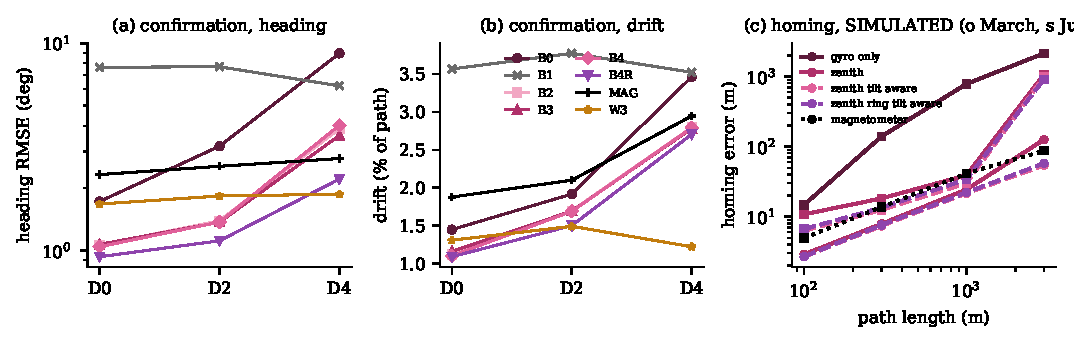
\includegraphics[width=\textwidth]{figs/fig_e03_results.pdf}
\caption{Study 3 results. (a, b) Confirmation split, trajectory level median heading RMSE and drift by level for the main systems (RENDERED images, SIMULATED compass). (c) SIMULATED homing error against path length for gyro only, the zenith compass with and without a tilt aware noise model, the zenith and ring compass (tilt aware) and the magnetometer, for a March morning (circles) and a June noon start (squares).}
\label{fig:s3res}
\end{figure*}

\subsection{Secondary analyses}
\textbf{Dust coupling.} The uncoupled and anchored runs use degradation seed 0 and one IMU draw; on that same seed and draw, coupling the sky to the image dust raises the B3 heading RMSE at D4 from \sunBthreeDfourhd{} to \scpsBthreeDfourhd{} degrees (B0 \scpsBzeroDfourhd{}), so it reduces the compass benefit by about \sbenefitRed{} percent (\sbenefitUn{} to \sbenefitCo{} degrees) but does not remove it, partly because the dust optical depth is capped at 10 by the table range. \textbf{Measured anchored sky.} With the clear sky DoP anchored to the Marseille measurement, B3 reaches \saBthreeDfourhd{} degrees and B4R \saBfourRDfourhd{} degrees at D4. \textbf{Other cues.} The assumed sun sensor is the best heading source at every level (\scSUNDzerohd{} to \scSUNDfourhd{} degrees) and the assumed magnetometer is flat across levels (\scMAGDzerohd{} to \scMAGDfourhd{} degrees) but worse than the sky compass with clear images because of its uncalibrated bias. \textbf{Variance.} For B3 at D2 and D4, the scenario (date, time, aerosol and cloud) explains \svcscen{} percent of the variance of log heading RMSE, the degradation seed \svctseed{} percent, the trajectory \svctraj{} percent and the environment \svcenvironment{} percent; \svcresidual{} percent is residual (IMU draw and interactions). A single degradation seed, as in Study~2, therefore understated the variation.

\subsection{Where the remaining drift comes from}
On the development split, an oracle heading (true yaw at 0.01 degrees) lowers the D4 drift from \sdevBzeroDfourdr{} to \sdevORHDfourdr{} percent, close to the compass systems, while an oracle translation (true body velocity, no compass) lowers the D0 drift from \sdevBzeroDzerodr{} to \sdevORTDzerodr{} percent. Once a compass is present, the residual drift is mostly visual translation error. That error is biased and wide (post hoc, development split): the visual forward speed has a median scale of \svoScaleDzero{} at D0 and \svoScaleDfour{} at D4, and an error standard deviation of \svoSdDzero{} m/s at D0, about four times the robust noise level the filter assumes. Neither oracle alone restores consistency (post hoc, development split): the median position NEES at D0, D2 and D4 is \sorORHDzeronees{}, \sorORHDtwonees{} and \sorORHDfournees{} with an oracle heading, \sorORTDzeronees{}, \sorORTDtwonees{} and \sorORTDfournees{} with an oracle translation, and \sorORXDzeronees{}, \sorORXDtwonees{} and \sorORXDfournees{} with both. Even the joint oracle stays overconfident, so part of the inconsistency lies in the inertial process model or in the oracle construction (velocities differentiated from poses); the biased visual translation is a candidate cause, not an established one, and a short correlation time scale state (B3C) cannot absorb a constant scale bias.

\subsection{Tilt}
\label{sec:tilt}
The rendered confirmation poses are level, so the frozen run has no tilt error. In a sensitivity run that applies the development tilt model (2 degrees, 20 s correlation) to the confirmation split (one IMU draw, one degradation seed), the compass still helps: B3 reaches \stBthreeDfourhd{} degrees at D4 against \stBzeroDfourhd{} for B0, and wheel odometry with the compass still drifts less than vision alone at D4 (\stWthreeDfourdr{} against \stBzeroDfourdr{} percent). The ring advantage, however, disappears: B4R reaches \stBfourRDzerohd{}, \stBfourRDtwohd{} and \stBfourRDfourhd{} degrees at D0, D2 and D4 against \stBfourDzerohd{}, \stBfourDtwohd{} and \stBfourDfourhd{} for B4, and the gated ring B3R is worse than both (\stBthreeRDtwohd{} degrees at D2). H4 therefore holds only for a level or tilt compensated sensor.


\subsection{Homing over kilometres (SIMULATED)}
In the homing study (wheel odometry and a gyro, 300 paths per case), the gyro alone reaches a median error of \shomMGyroonek{} m after 1 km. With the zenith compass and a tilt aware noise model the error after 3 km is \shomMZenTAthreek{} m on a March morning but \shomJZenTAthreek{} m when the drive crosses the June noon window, against \shomMMagthreek{} m for the assumed magnetometer. Without a tilt aware noise model the ring compass is gated out by tilt and loses its advantage (\shomMRingthreek{} m after 3 km in March). The growth exponents (position error against path length) lie between about 0.85 and 1.6, so any extrapolation to 10 km is a model statement only.
